\todo[inline]{I don't think the terms traffic assignment and route choice are used interchangeably}
\ggnote{I was looking at this: \url{https://en.wikipedia.org/wiki/Route_assignment}}
The term \textit{traffic assignment} (or route choice, or route assignment) captures a large array of problems concerning the distribution of traffic over a network. Traffic assignment problems arise in transportation planning applications, such as in the traditional ``four-step'' procedure, where it occupies the final step, following trip generation, trip distribution, and mode choice \cite{mcnally2007four}.  The fundamental principle that guides most traffic assignment models is Wardrop's principle \cite{wardrop1952some}, which states that amongst the available alternatives, drivers will select routes that minimize their travel times. Because the speed of traffic tends to decrease as the number of vehicles on the route increases, Wardrop's principle leads to an iterated game in which drivers test new routes, day after day, until they converge to a Nash equilibrium, a.k.a. a \textit{user equilibrium}. The term is also used for problems that involve a single decision maker, who prescribes the routes for users in order to optimize some system-level performance metric, e.g. total travel time, emissions, energy consumption. These are mathematical programs, and their solutions are known as \textit{system optimal} assignments. We will focus in this paper on user equilibrium traffic assignments. \todo[inline]{might be nice to specify Wardrop's 1st and 2nd principles}

Since the pioneering work of Wardrop, the mathematical and numerical study of traffic assignment has progressed at a moderate pace. \todo[inline]{"moderate pace" seems weird. like as opposed to fast? what is fast? what is slow?} \ggnote{Id like to say that it has progressed very slowly.}
This is perhaps mostly due to a historical scarcity of traffic data and network information, but also because of the difficulty of the problem. [CCC] gives several examples in which problems could not be solved for networks of useful size. It is not surprising therefore that the problem has received renewed interest with recent increases in traffic and network data, and computational power. Also driving this renewal are concerns about the `unintended consequences' of the widespread use of routing apps \cite{traffic_apps}, as well as advances in autonomous driving technologies.

An investigation into the techniques of traffic assignment reveals a multitude of traffic flow models, numerical methods, and performance metrics. \todo[inline]{when we say "models" we are referring to models of traffic flow dynamics - is it clear to just say "models"?} \ggnote{fixed.} As is usually the case, the more detailed the model, the more expensive the computation. However it is not clear under which circumstances the additional effort (or investment in computational resources) is necessary. For example, although it is usually agreed that dynamical models that capture the essential phenomenon of congestion are desirable, it is also true that the computation (as well as network configuration effort) involved in solving dynamic traffic assignment (DTA) problems can be large. On the other hand, existing static planning methods cannot fully model traffic congestion because of their inability to represent queue formation and dissipation when traffic demand exceeds road capacities\cite{nie2010solving}. 

This paper presents a software framework for addressing such questions. The software is based on the formulation of traffic assignment as a \textit{variational inequality}, introduced by Nagurney \cite{nagurney2013network}. This is a very general formulation, as it requires only continuity (\XXX TRUE?) of the traffic model. Hence, it covers a wide range of models: static and dynamic, macroscopic and microscopic, `analytical' and `simulation-based', etc. The software is modular and extensible, in the sense that it provides interfaces for incorporating new models, cost functions, and numerical solvers. 

There are many other programs, both commercial and shared, that solve dynamic traffic assignment problems. 

\ggnote{I want to de-emphasize the analytical vs simulation-based dichotomy because I don't understand it. Is beats analytical or simulation-based. If simulation-based, then CTM is simulation-based? Most people would disagree, because the line is very fuzzy, and really the distinction makes little sense (as our framework demonstrates). Instead lets focus on modularity: All others (I hope) bake in the model, cost function, and solver.}

\ggnote{The list needs to be fleshed out a bit. For each, can we answer these questions: what is the problem being solved? What is the model? What is the solver algorithm? Then we can categorize them in some way.}


\todo[inline]{Should we include microsims? If yes - many to add from Fund. of Traffic Sim. book. If no - remove INTEGRATION}
\todo[inline]{Make formatting better}
\begin{table}
    \centering
    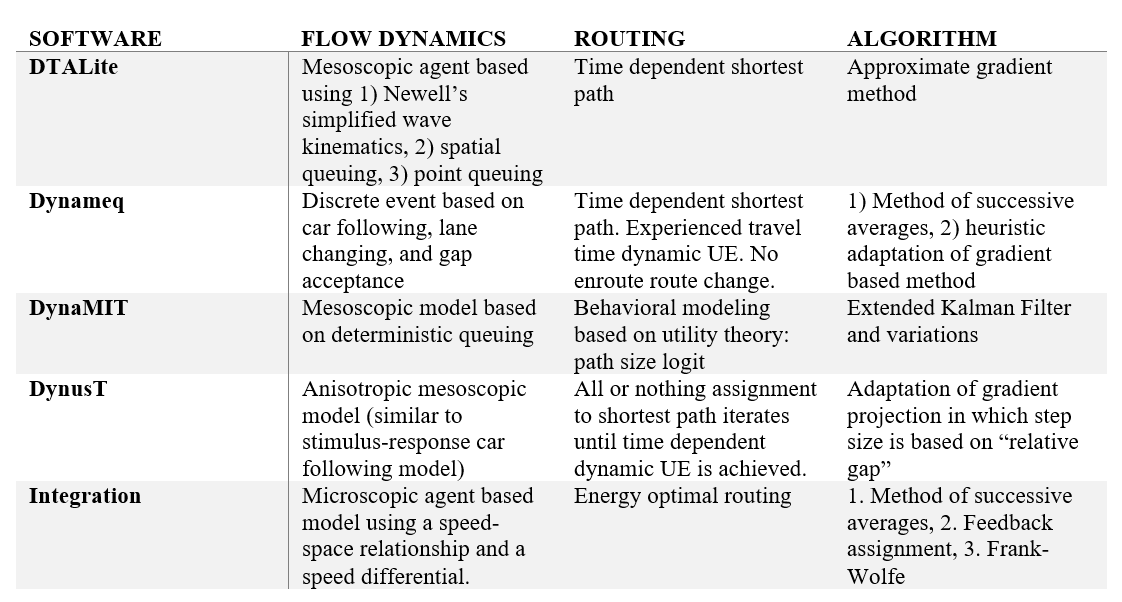
\includegraphics[width=0.5\textwidth]{figs/lit_table.PNG}
    \caption{}
    \label{tab:times}
\end{table}

\begin{itemize}
\item DTALite \cite{zhou2014dtalite} uses a mesoscopic agent based model with link flow dynamics based on Newell’s simplified kinematics wave model, a spatial queue model, and a point queue model. Node dynamics are governed by signal timing, Daganzo’s priority based merging, and flow conservation. Initial routing is based on time dependent shortest paths although utility theory and other traffic assignment rules can also be incorporated. DTALite uses an approximate gradient method solver which uses a queue model to calculate link flow–density change due to incoming path flow change. DTALite uses agent-based algorithm to calculate dynamic traffic equilibrium.
\ggnote{\url{https://www.tandfonline.com/doi/full/10.1080/23311916.2014.961345#} Mesoscopic model, assumes link flows are observed, solve an optimization problem to match path flows to observed link flows (Section 4.1 in reference?). Has no equilibrium concept} 
\item Dynameq uses a discrete event traffic flow model in contrast to the more typical discrete time based models. The model is based on car following, lane changing, and gap acceptance. Initial routing is done by time dependent shortest path and convergence to experienced travel time dynamic user equilibrium is sought. Vehicles do not change paths enroute, instead they follow initially designated routes. Two solver algorithms are employed: 1) the method of successive averages and, 2) a heuristic adaptation of a gradient based method.   
\item DynaMIT-P \cite{DynaMIT,ben2001dynamit} is a mesoscopic model based on speed-density relationships and queuing theory. Route choice behavior is based on utility theory and a path size logit model is used. Joint estimation of unknown state space parameters (including OD flow, route choice model parameters, traffic dynamic model parameters, and segment capacities) is conducted using an Extended Kalman Filter and other variations of Kalman filtering.   \ggnote{Section 3: \url{https://www.sciencedirect.com/science/article/pii/S1474667017438572}}
\item DYNASMART-P \cite{DYNASMART,mahmassani2004dynasmart} is a simulation-based DTA tool based on the the mesoscopic traffic simulator DYNASMART. 
\item DynusT \cite{chiu2011dynust} uses the “anisotropic mesoscopic model” for flow dynamics which is similar to a stimulus-response type of car following model in which the two defining features are 1) a vehicle’s speed is influenced by vehicles in front of it (in same lane and adjacent lanes), and 2) the influence of downstream traffic decreases as distance increases. The time dependent shortest path algorithm determines the time-dependent shortest path for each departure time. The traffic assignment assigns a portion of the vehicles departing at the same time between the same OD pair to the time-dependent least-travel time path following the “route swapping” type of traffic assignment procedure. The solution algorithm is based on an adaptation of gradient projection in which the step size is based on “relative gap” which is a measure of the difference between experienced travel time and time dependent shortest path travel time. 
\item INTEGRATION \cite{rakha2012integration} uses a microscopic agent based flow model based on speed-spacing relationships, a speed differential between a vehicle and the vehicle immediately ahead of it, and an acceleration model (variable power vehicle dynamics model) that considers the vehicle’s tractive force. The authors of INTEGRATION jointly consider routing and solution algorithms. Their software incorporates: 1) time dependent method of successive averages, 2) time dependent sub-population feedback assignment, 3) time dependent agent feedback assignment, 4) time dependent dynamic traffic assignment, 5) time dependent Frank-Wolfe algorithm, 6) time dependent external routing, and 7) distance based routing.  

\end{itemize}

In contrast to these, the software described here does not prescribe the model, cost-function, or numerical method, but rather serves as a platform for comparing different options, both in terms of computation and the solutions they produce. The software presently includes a static model, two dynamic models: the cell-based model and the Merchan-Nemhouser model, a travel time based cost-function, and three numerical algorithms: the Frank-Wolfe algorithm, the method of successive averages, and the extra-projection method. The code can be found here \cite{ta_solver}. \ggnote{Briefly mention the items we've implemented so far - addressed, Juliette}


%%%%%%%%%%%%%%%%%%%%%%%%%%%%%%%%%%%%%%%%%%%%%%%%%%%

% In addition, VI's extension and sensitivity analysis can be conveniently performed \cite{peeta2001foundations}. 
% [GG: This sounds like it might be important, but I am not sure what it is, or if it compares favorably to other sensitivity analyses, eg lagrange multipliers in optimization problems]

% Though the theory of DTA is still relatively undeveloped, variational inequality (VI) has proven to provide a unified formulation to address various classes of equilibrium and equivalent optimization problems in the DTA context. 
% [GG: I incorporated this idea in the text]
 
%Static methods were developed for long term transportation planning and are not applicable in dynamic route guidance systems that require the ability to solve transportation problems in real time\cite{boyce1989route}. 
% [GG: This is too strong of an assertion for my taste]

% In recent years, dynamic traffic assignment (DTA) has gained heightened interest, as researchers and practitioners are recognizing the need to predict the spatio-temporal evolution of traffic and the limitations of  static traffic assignment methods\cite{peeta2001foundations}. 
% [GG: The reference here is too old to be recent. Is there something more recent?]

% In this paper, we extend VI formulation to unify analytical DTA models with simulation-based DTA models. 
% [GG: I dont want to say that we did it, because most people wouldnt consider CTM a simulation. I'd rather say that we created a framework that will support it.]

% Simulation-based DTA methods compliment analytical techniques by addressing the shortcomings of analytical link models and exit functions in reproducing dynamic traffic interactions, satisfying First-In-Fist-Out property, and replicating complex vehicles and multi-user class interactions. 
% [GG: The line between "analytical" and "simulation-based" is artificial. I think we should move beyond and speak at a higher level than that false debate. I dont understand the difference between "analytical" and "simulation-based" anyway.]

% VI formulations can model more realistic traffic scenario by bypassing the issues of solution intractability associated with other analytical DTA methods such as mathematical programming and optimal control formulations. 
% [GG: This is not true.]


% our software is the first to combine simulation-based DTA models with analytical methods including mathematical programming and optimal control into one software platform. In addition, our software framework is based on a clear underlying VI DTA formulation. The general VI formulation determines the overall software architecture, but also provide a way to incorporate any type of DTA problem that can be represented with VI. 
% [GG : I really would rather not make grand claims. The clarity we've gained is only relative to my ignorance when we started. But there are people for whom everything we say here is obvious.]